\chapter{Gas de fermi de electrones libres} \label{Ch:06}

En este capítulo se comienza el estudio de los metales con un primer modelo en el que los electrones de valencia de los átomos del metal se \textit{independizan} cosntituyéndose en electrones de conducción que se mueven de una forma casi completamente libre a través del metal. De manera más precisa se supone que la red de iones positivos en el metal está inmóvil (red \textit{fría}) y además se sustituye por un fondo positivo de carga (a veces llamado \textit{modelo jalea}) de modo que el potencial eléctrico a que están sometidos los electrones de conducción es una constante que puede tomarse como cero. Se admite además que los electrones no interaccionan entre sí, pero debido a su carácter fermiónico les aplicaremos el Principio de Exclusión de Pauli. Hablaremos entonces de \textit{Gas de Fermi de elctrones libres}.

\section{Estados fundamentales del gas de Fermi}

\subsection{Niveles de energía}

Por tratarse de electrones independientes debemos calcular los niveles de un solo electrón, que luego serán ocupados por todos los electrones libres del metal: es la \textit{aproximación monoeléctrica}. Consideremos pues un electrón libre en un volumen $V=L_1L_2L_3$. La función de onda es, como es sabido, 

\begin{equation}
    \psi_\kn = V^{-1/2} e^{i \kn \cdot \rn} \label{Ec:06-01-01}
\end{equation}
con energía e impulso, respectivamente 

\begin{equation}
\begin{array}{ccc}
    \epsilon & = &\hbar^2 k^2 /2m \\
    \pn &= &  \hbar \kn
\end{array}
\end{equation}
Se aplican ahora a (\ref{Ec:06-01-01}) las condiciones de contorno periódicas:

\begin{equation}
    \begin{array}{ccc}
    \psi_\kn (x,y,z+L_3) & = & \psi_\kn (x,y,z) \\
    \psi_\kn (x,y+L_2,z) & = & \psi_\kn (x,y,z) \\
    \psi_\kn (x+L_1,y,z) & = & \psi_\kn (x,y,z) \\
    \end{array}
\end{equation}
que conducen a 
\begin{equation}
    k_i = n_i 2 \pi / L_i \quad (i=1,2,3 \ \text{y} \ n_i \in \mathbb{Z})
\end{equation}
De esta forma el volumen del espacio recíproca asociado a cada valor posible de $\kn$ es $8\pi^3 /V$, con densidad uniforme. Si ahora tenemos $N$ electrones para ``colocar'' el estado fundamental a $T=0$K consiste en ir llenando por energías crecientes los distintos estados monoelectrónicos respetando el Principio de Exclusión hasta agotar los $N$ electrones. La situación final es como se esquematiza en la figura \ref{Fig:06-01} (cada punto corresponde a dos electrones).

\begin{figure}[h!] \centering
    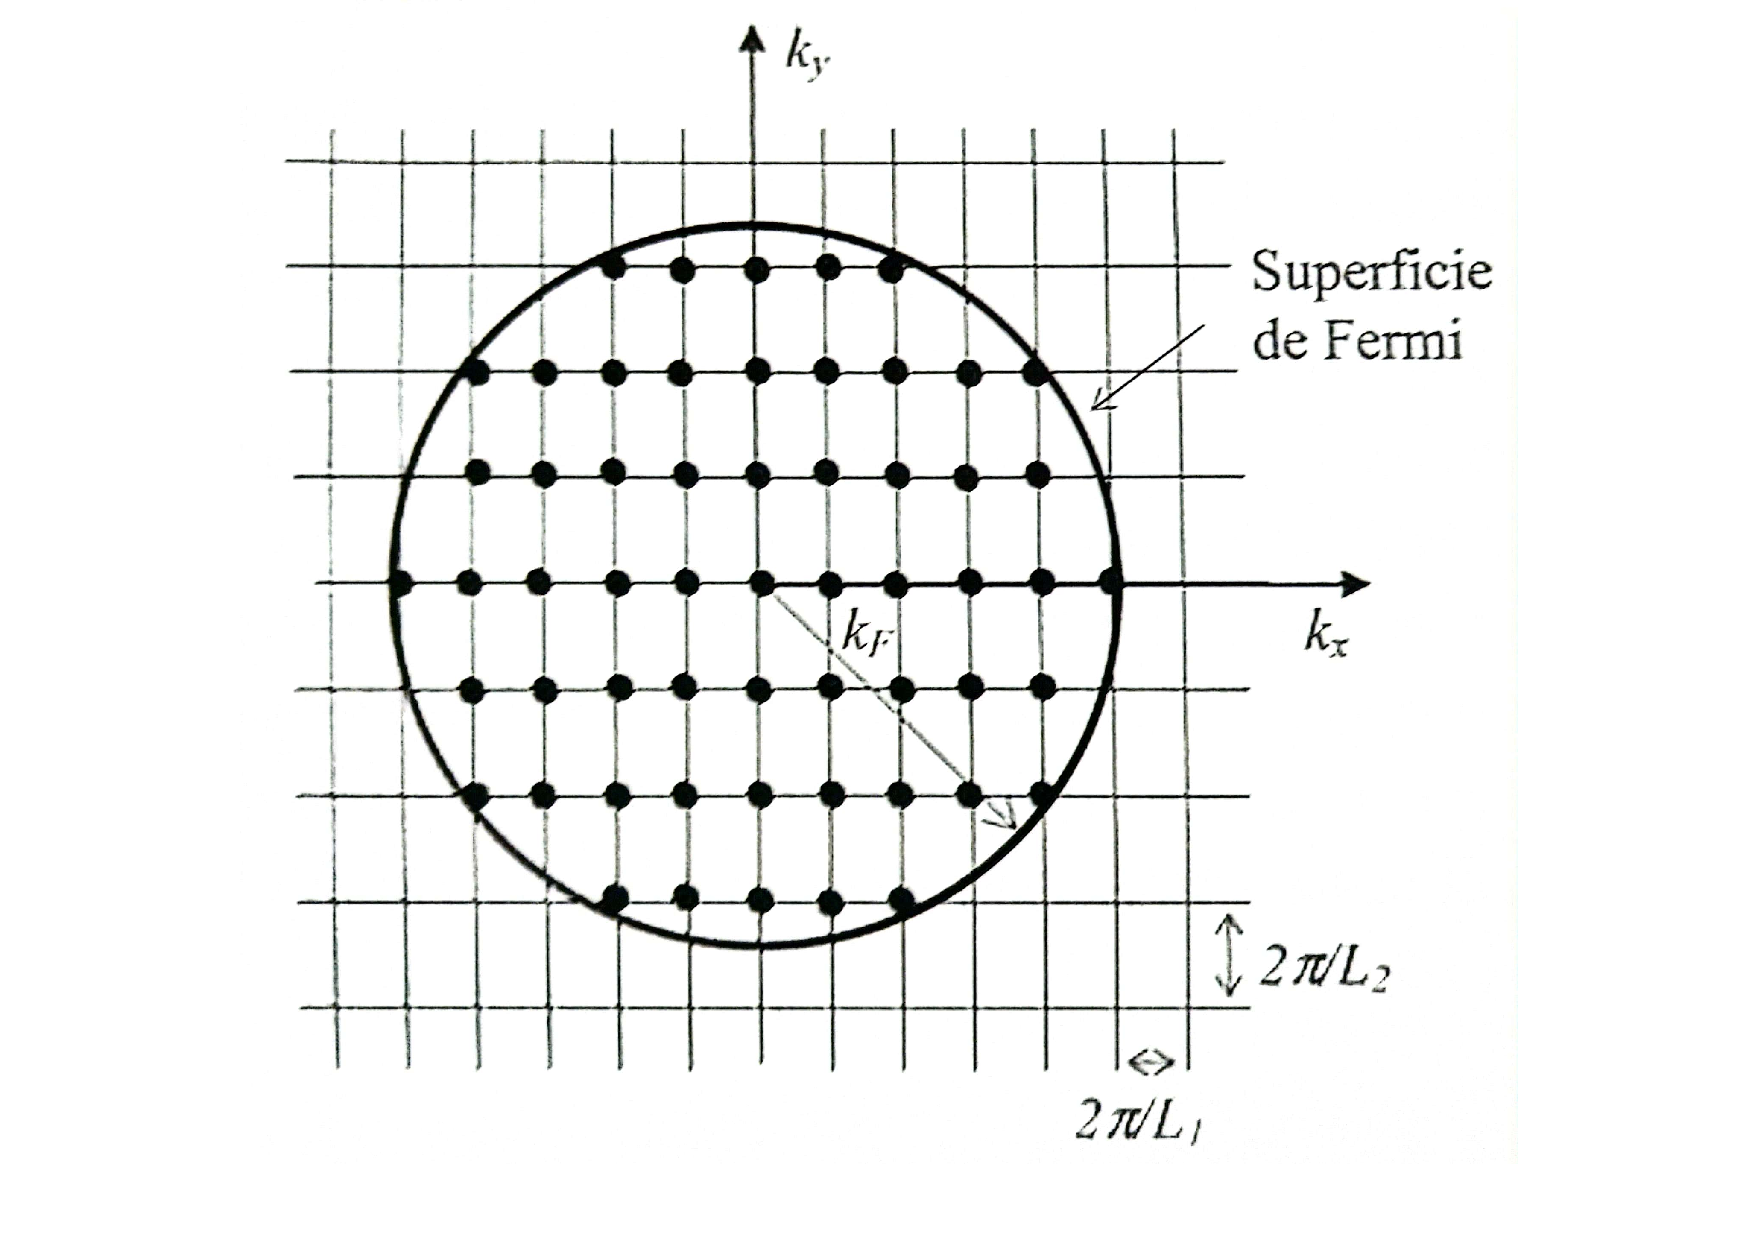
\includegraphics[scale=0.35]{Cuerpo/Ch_06/Fotos libro 1.pdf}
    \caption{Distribución de estados electrónicos ocupados en el espacio de fases.}
    \label{Fig:06-01}
\end{figure}    

La \textit{superficie de Fermi} es la superficie que separa los estados ocupados de los desocupados. A continuación vamos a definir los términos de Fermi:

\begin{itemize}
	\item \textbf{Vector de onda de Fermi (3D):}
	\begin{equation}
		k_F = (3\pi^2 n)^{1/3} \quad (n\equiv N/V) \label{Ec:06-01-05}
	\end{equation}
	\item \textbf{Vector de onda de Fermi (2D):}
	\begin{equation}
		k_F= \sqrt{2\pi n}
	\end{equation}
	\item \textbf{Energía de Fermi:}
	\begin{eqnarray}
		\varepsilon_F \equiv \frac{\hbar^2 k_F^2}{2m} \label{Ec:06-01-07}
	\end{eqnarray}
	\item \textbf{Velocidad de Fermi:}
	\begin{eqnarray}
	v_F \equiv \sqrt{2\varepsilon_F /m}
	\end{eqnarray}
	\item \textbf{Temperatura de Fermi:}
	\begin{eqnarray}
		T_F \equiv k_B \varepsilon_F
	\end{eqnarray}
\end{itemize}
Todos estos parámetros dependen sólo de la concentración electrónica $n$ uqe es conocida para metales: $10^{22}<n(\textbf{cm}^{-1})<10^{23}$. Numéricamente, resultan los siguientes valores:

\begin{equation*}
	\begin{array}{c}
	\varepsilon_F = 1-10 \unit{\eV} \\
	T_F = 10^4 - 10^5 \unit{K} \\
	v_F = (0.7-2)\times 10^8 \unit{\cm/s}\\
	v_F = (0.7-1.7)\times 10^8 \unit{\cm^{-1}}
	\end{array}
\end{equation*}
La \textbf{densidad de estados} $D(\varepsilon)$ se calculaa fácilmente haciendo referencia a la figura \ref{Fig:06-02}, resultando:

\begin{equation}
	D(\varepsilon) \D \varepsilon = 2 \times \frac{4\pi k^2 \D k}{8 \pi3 /V} = \frac{V}{2\pi2} \parentesis{\frac{2m}{\hbar2}}^{3/2} \sqrt{\varepsilon} \D \varepsilon \label{Ec:06-01-10}
\end{equation}
El factor $2$ da cuenta de los dos estados electrónicos posibles. Es útil expresar la densidad de estados $D(\varepsilon)$ en función de $\varepsilon_F$ combinando (\ref{Ec:06-01-10}), con (\ref{Ec:06-01-05}) y (\ref{Ec:06-01-07}) resulta:

\begin{equation}
	D(\varepsilon) = \frac{3}{2} \frac{N}{\varepsilon_F} \sqrt{\frac{\varepsilon}{\varepsilon_F}} \label{Ec:06-01-11}
\end{equation}	

A menudo es más útil trabajar con el número de estados por unidad de volumen del cristal, en cuyo caso basta hacer en (\ref{Ec:06-01-12}) la sustitución $N\rightarrow N/V=n$.
	
\begin{figure}[h!] \centering
    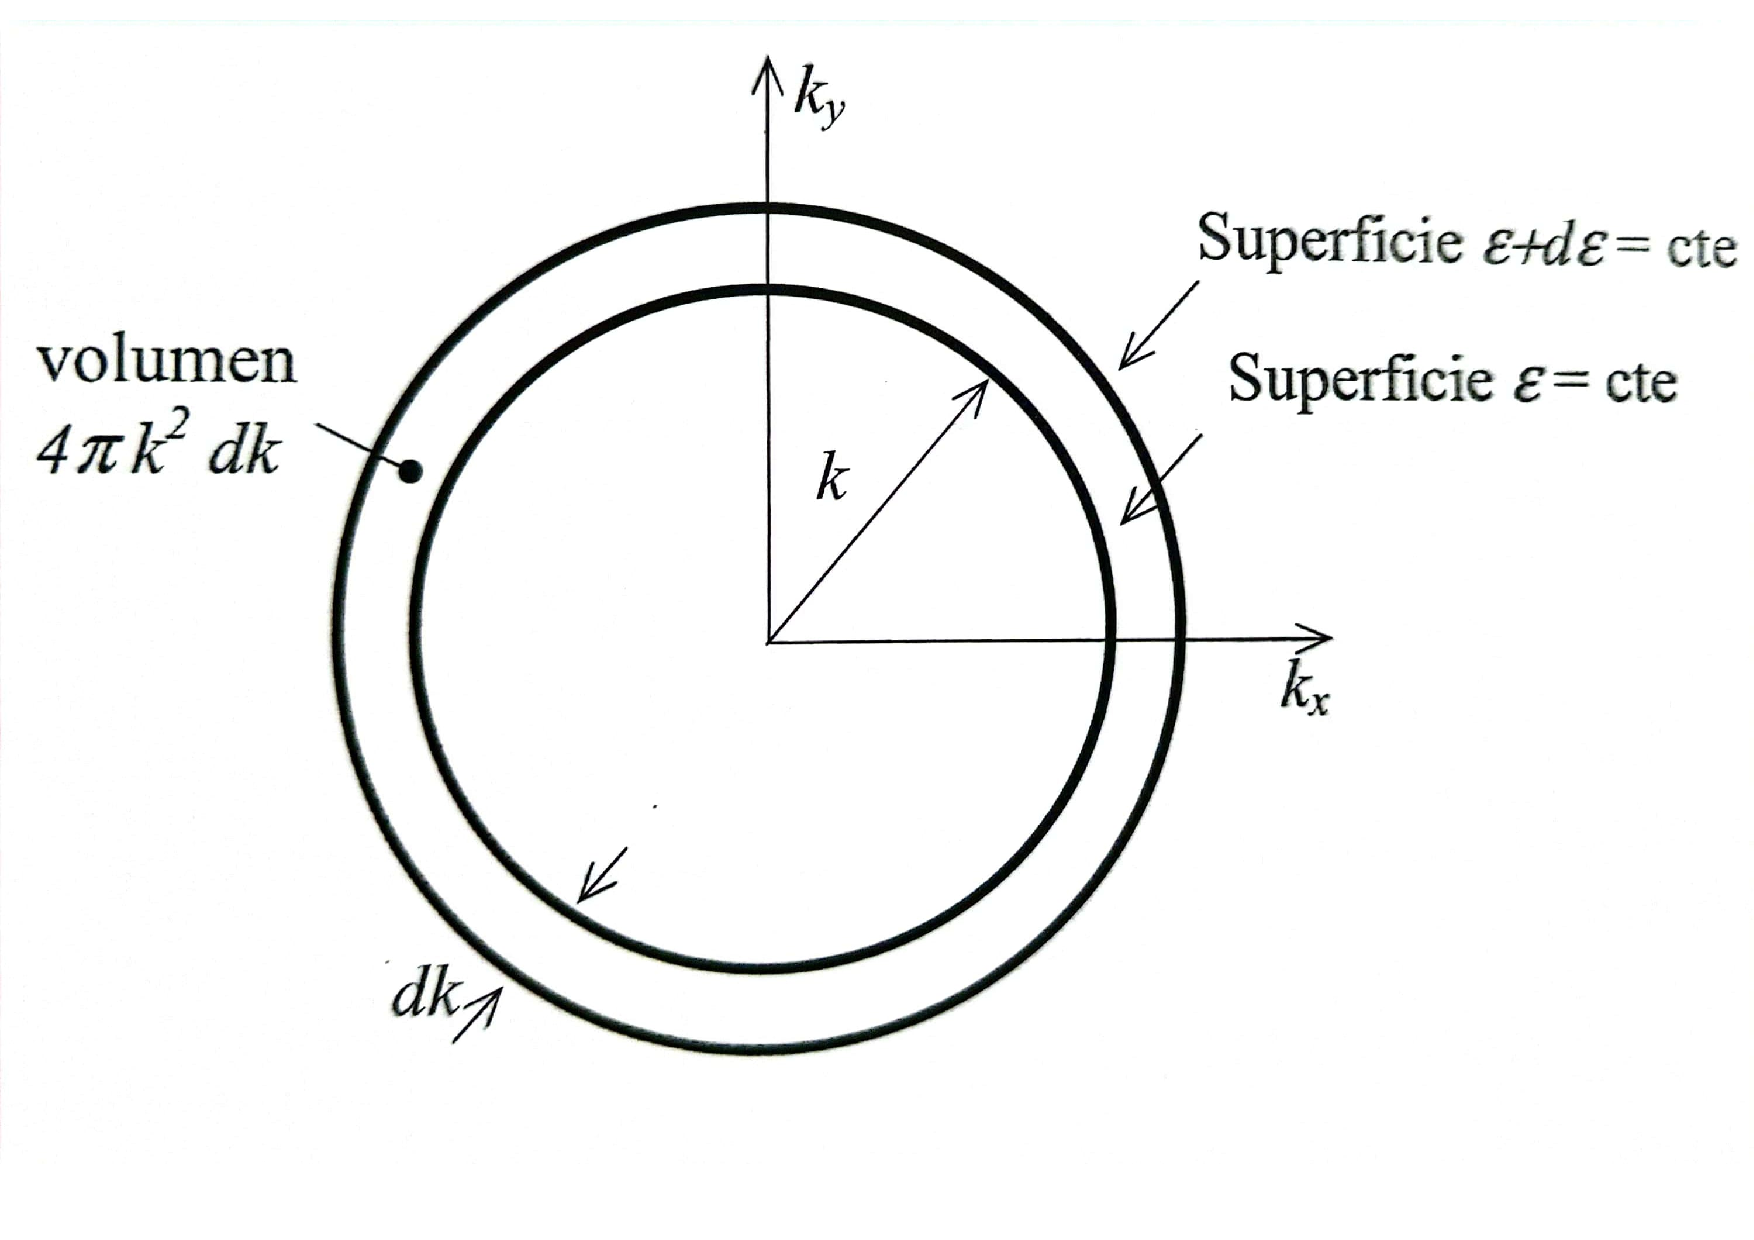
\includegraphics[scale=0.35]{Cuerpo/Ch_06/Fotos libro 2.pdf}
    \caption{Cálculo de la densidad de estados electrónicos.}
    \label{Fig:06-02}
\end{figure}  

\subsection{Ocupación de estados a $T>0$}

Se trata de saber cómo cambia el llenado de estados si el gas de electrones está a una temperatura finita. Por tratase de fermiones la respuesta la da la distribución de Fermi-Dirac, según la cual la probabilidad $f_{FD}$ de que un estado $\kn$ esté ocupado es:

\begin{equation}
	f_{FD} (\kn) = \frac{1}{e^{(\varepsilon(\kn)-\mu)/k_B T} +1}  \label{Ec:06-01-13}
\end{equation}
donde $\mu$ es el potencial química que verifica $f_{FD}(\mu)=1/2$. A $T=0$K, como esperaríamos, $f_{FD}(\varepsilon<\mu)=1$ y $f_{FD}(\varepsilon>\mu)=0$, por lo que podemos decir que $\varepsilon_F=\mu(T=0\textbf{K})$. A $T>0$ K la función $f_{FD}$ tiene el perfil que se grafíca en la figura \ref{Fig:06-03}. El potencial químico de la ligadura:

\begin{equation}
	N=\int_0^{\infty} f_{FD} (\varepsilon) D (\varepsilon) \D \varepsilon  \label{Ec:06-01-14}
\end{equation}
Al sustituir (\ref{Ec:06-01-12}) y (\ref{Ec:06-01-13}) en (\ref{Ec:06-01-14})  resulta una integral no analítica. Gracias a que $T\ll T_F$ las integrales de tipo (\ref{Ec:06-01-14}) se pueden aproximar por la llamada \textit{expansión de Sommerfeld} 

\begin{eqnarray}
	\int_{0}^{\infty} H(\varepsilon) f_{FD} (\varepsilon)  \D \varepsilon \approx \int_0^\mu H(\varepsilon) \D \varepsilon + \frac{\pi2 k_B^2 T^2}{6} \derivadas{\D H}{\D \varepsilon} (\mu)
\end{eqnarray}
Aplicando esta relación a (\ref{Ec:06-01-14}), tras alguna manipulación se llega a 

\begin{equation}
	\mu (T) = \mu(0) \ccorchetes{1-\frac{1}{3} \parentesis{\frac{\pi T}{2 T_F}}^2}
\end{equation}
 



\begin{figure}[h!] \centering
    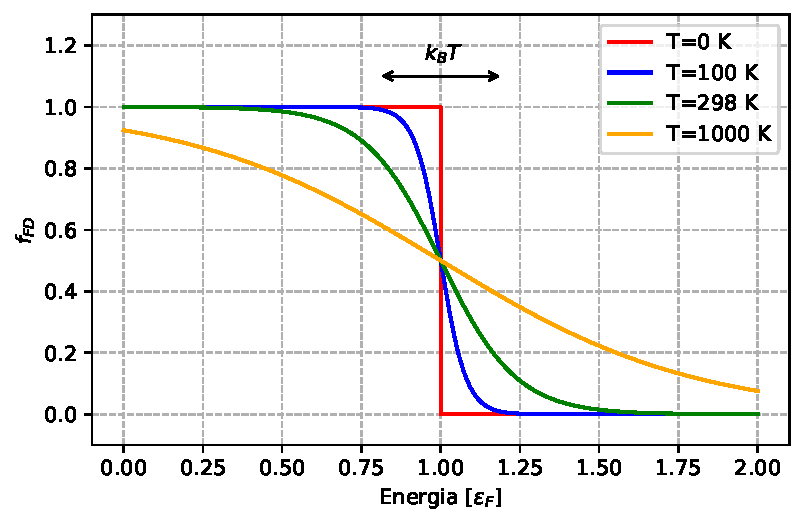
\includegraphics[scale=0.75]{Cuerpo/Ch_06/06-Fermi-Dirac.pdf}
    \caption{Distribución de Fermi-Dirac.}
    \label{Fig:06-03}
\end{figure}    

\subsection{Interacción electrón-electrón}

\begin{figure}[h!] \centering
    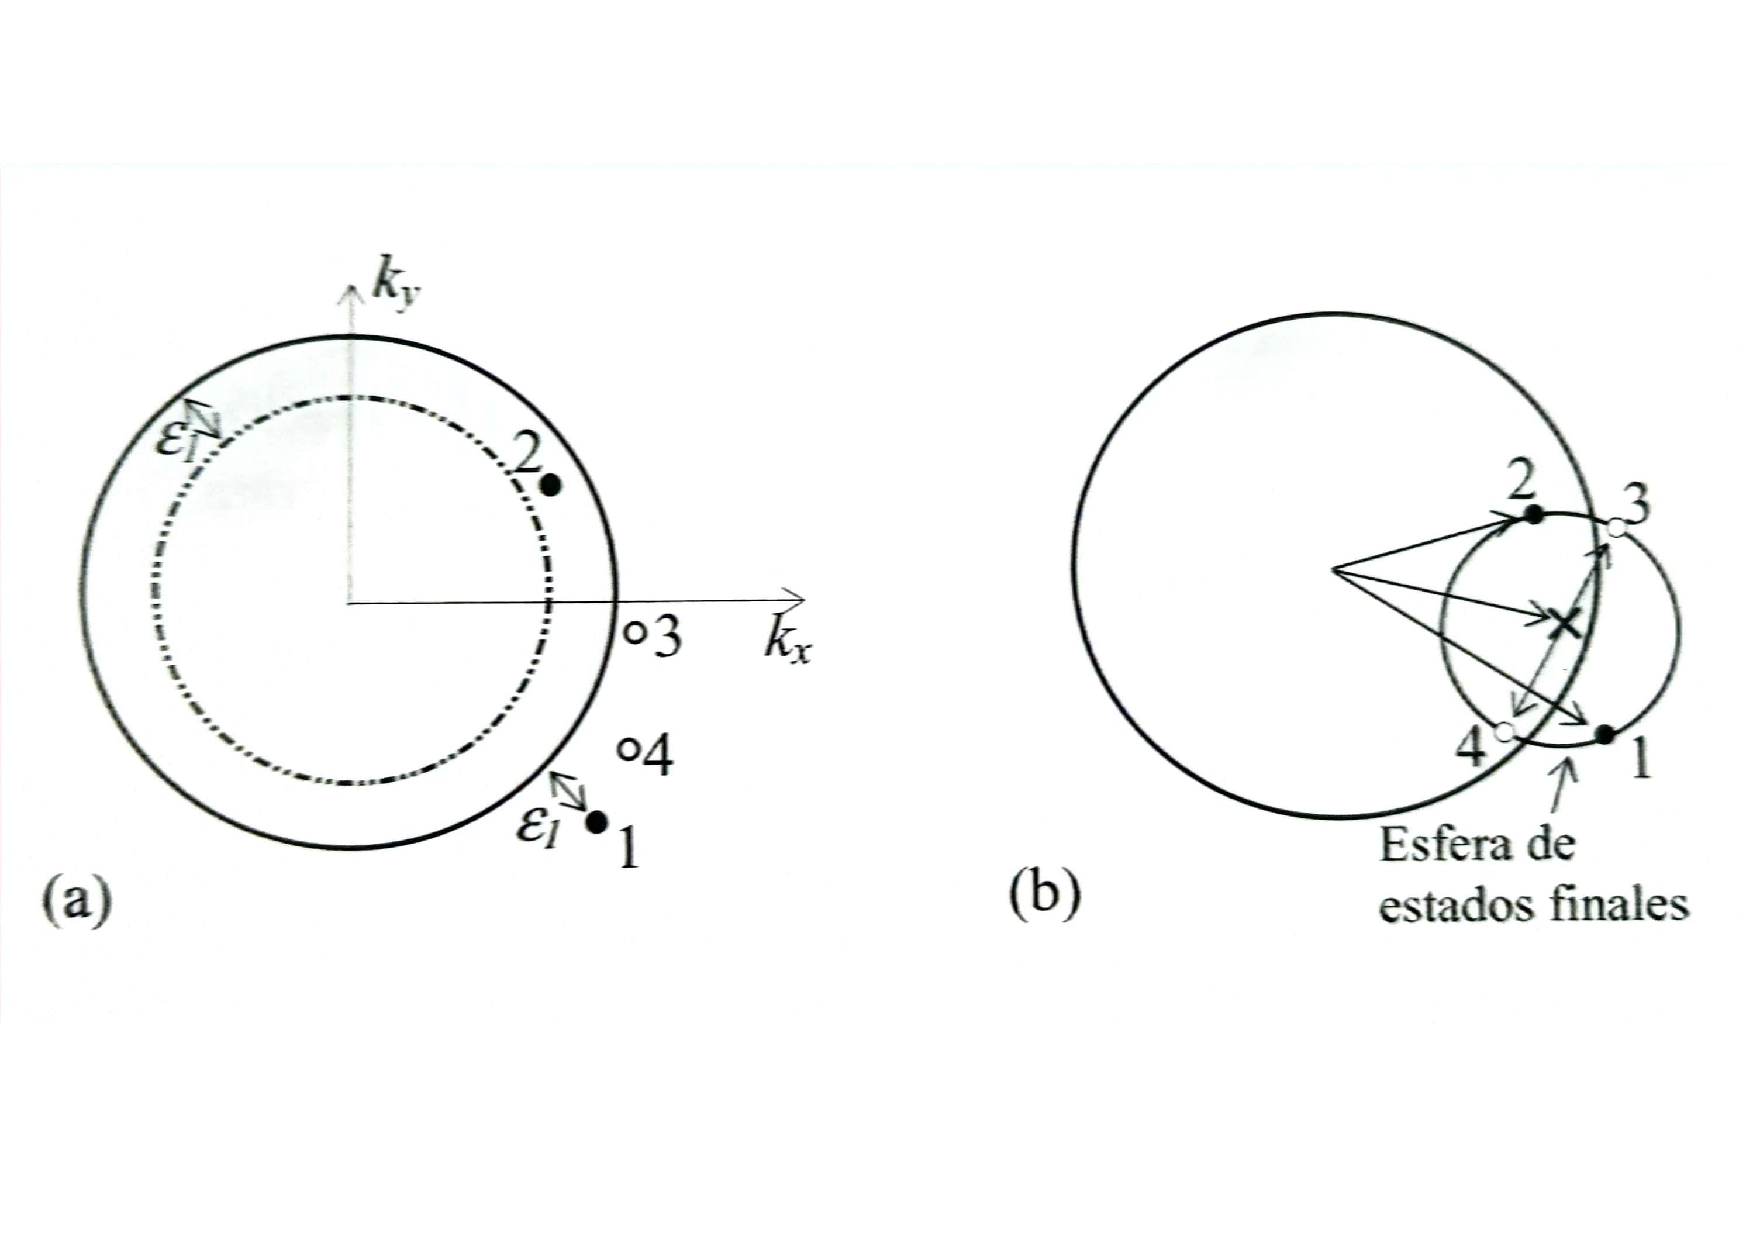
\includegraphics[scale=0.5]{Cuerpo/Ch_06/Fotos libro 4.pdf}
    \caption{Restricción a los procesos de colisión $e^- - e^-$ debido a las leyes de conservación de la energía (a) y del momento (b).}
    \label{Fig:06-04}
\end{figure}  

\section{Capacidad térmica electrónica}

\section{Conductividad eléctricca DC}

\subsection{Modelo cinético de Drude y ecuación dinámica}

\subsection{Ley de Ohm}
\begin{figure}[h!] \centering
    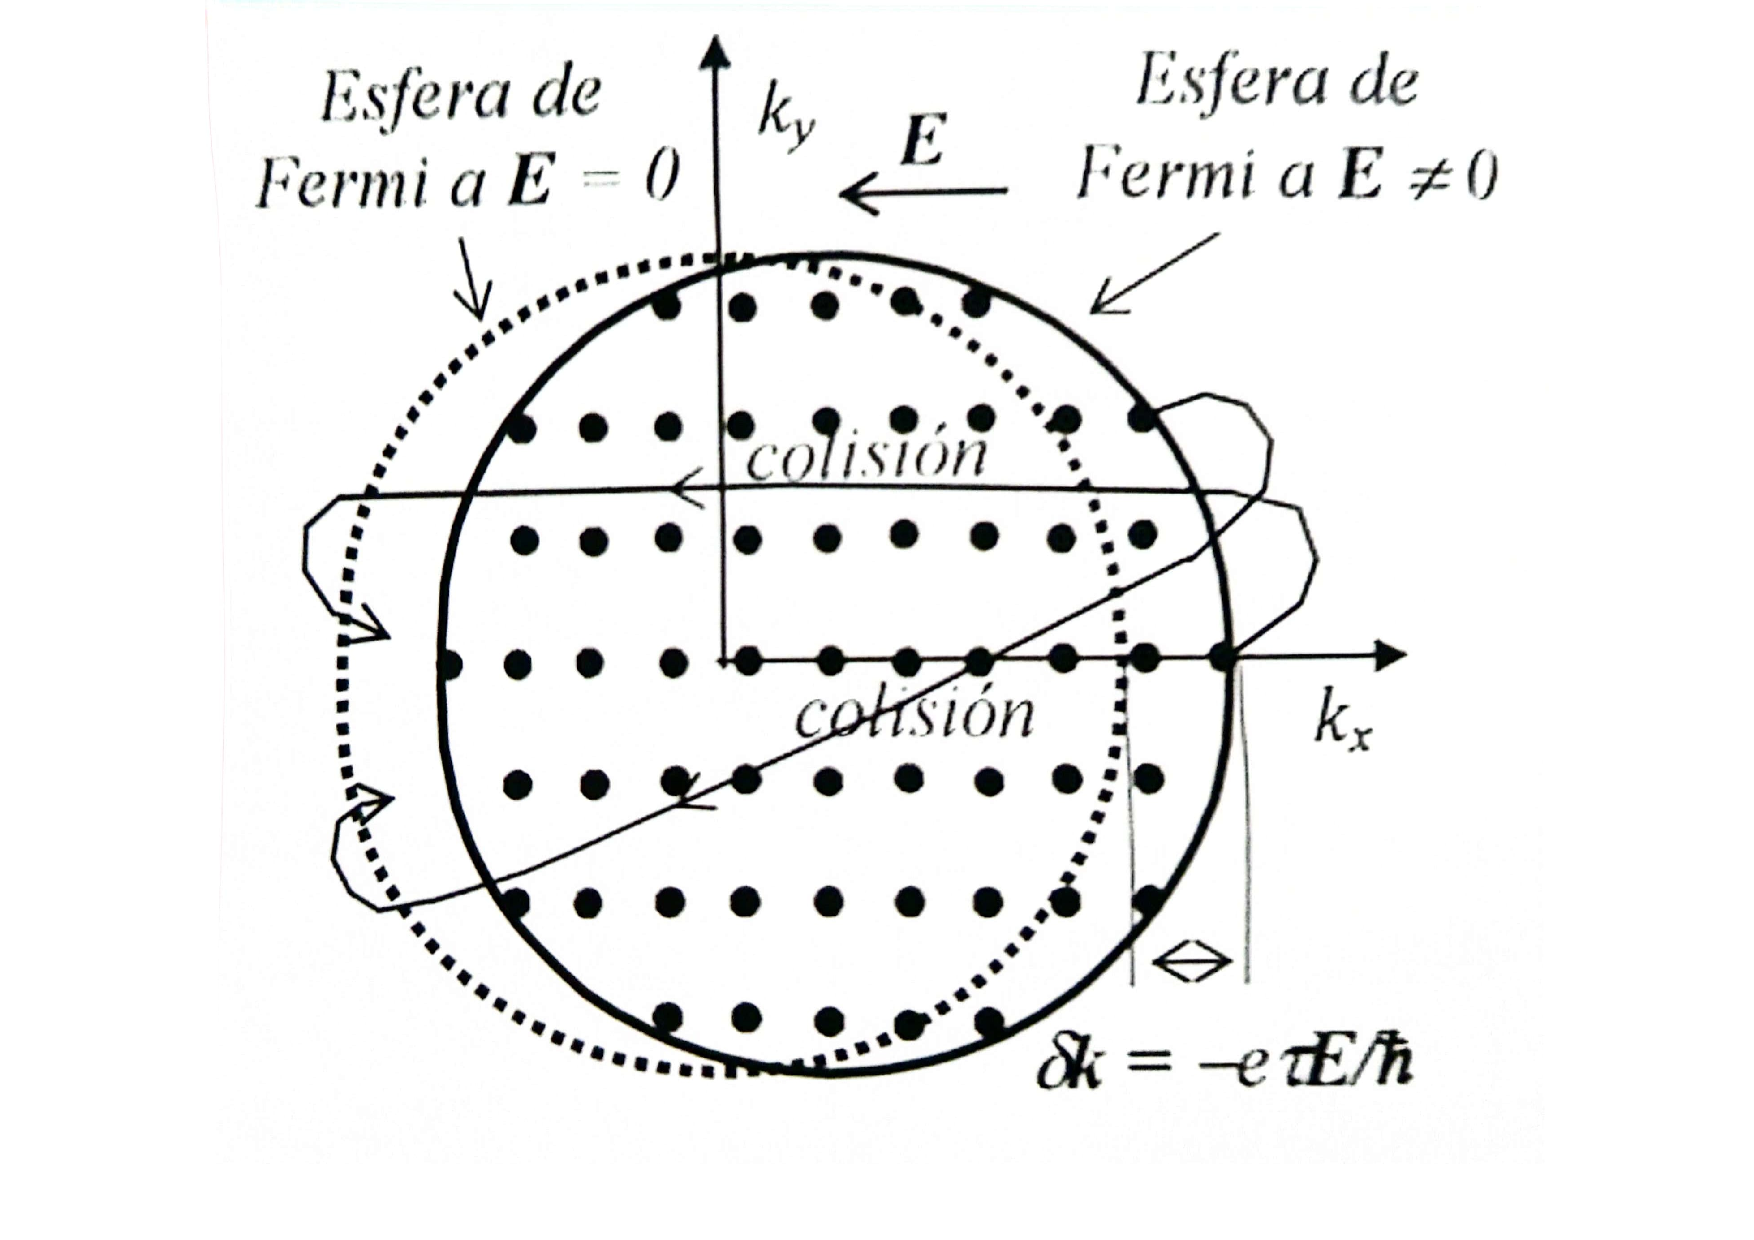
\includegraphics[scale=0.5]{Cuerpo/Ch_06/Fotos libro 5.pdf}
    \caption{Desplazamiento de la ``esfera de Fermi'' bajo la aplicación de un campo eléctrico. Las líneas indican algunos procesos de colisión permitidos.}
    \label{Fig:06-05}
\end{figure}  

\subsection{Dependencia con la temperatura de la conductividad eléctrica}
\begin{figure}[h!] \centering
    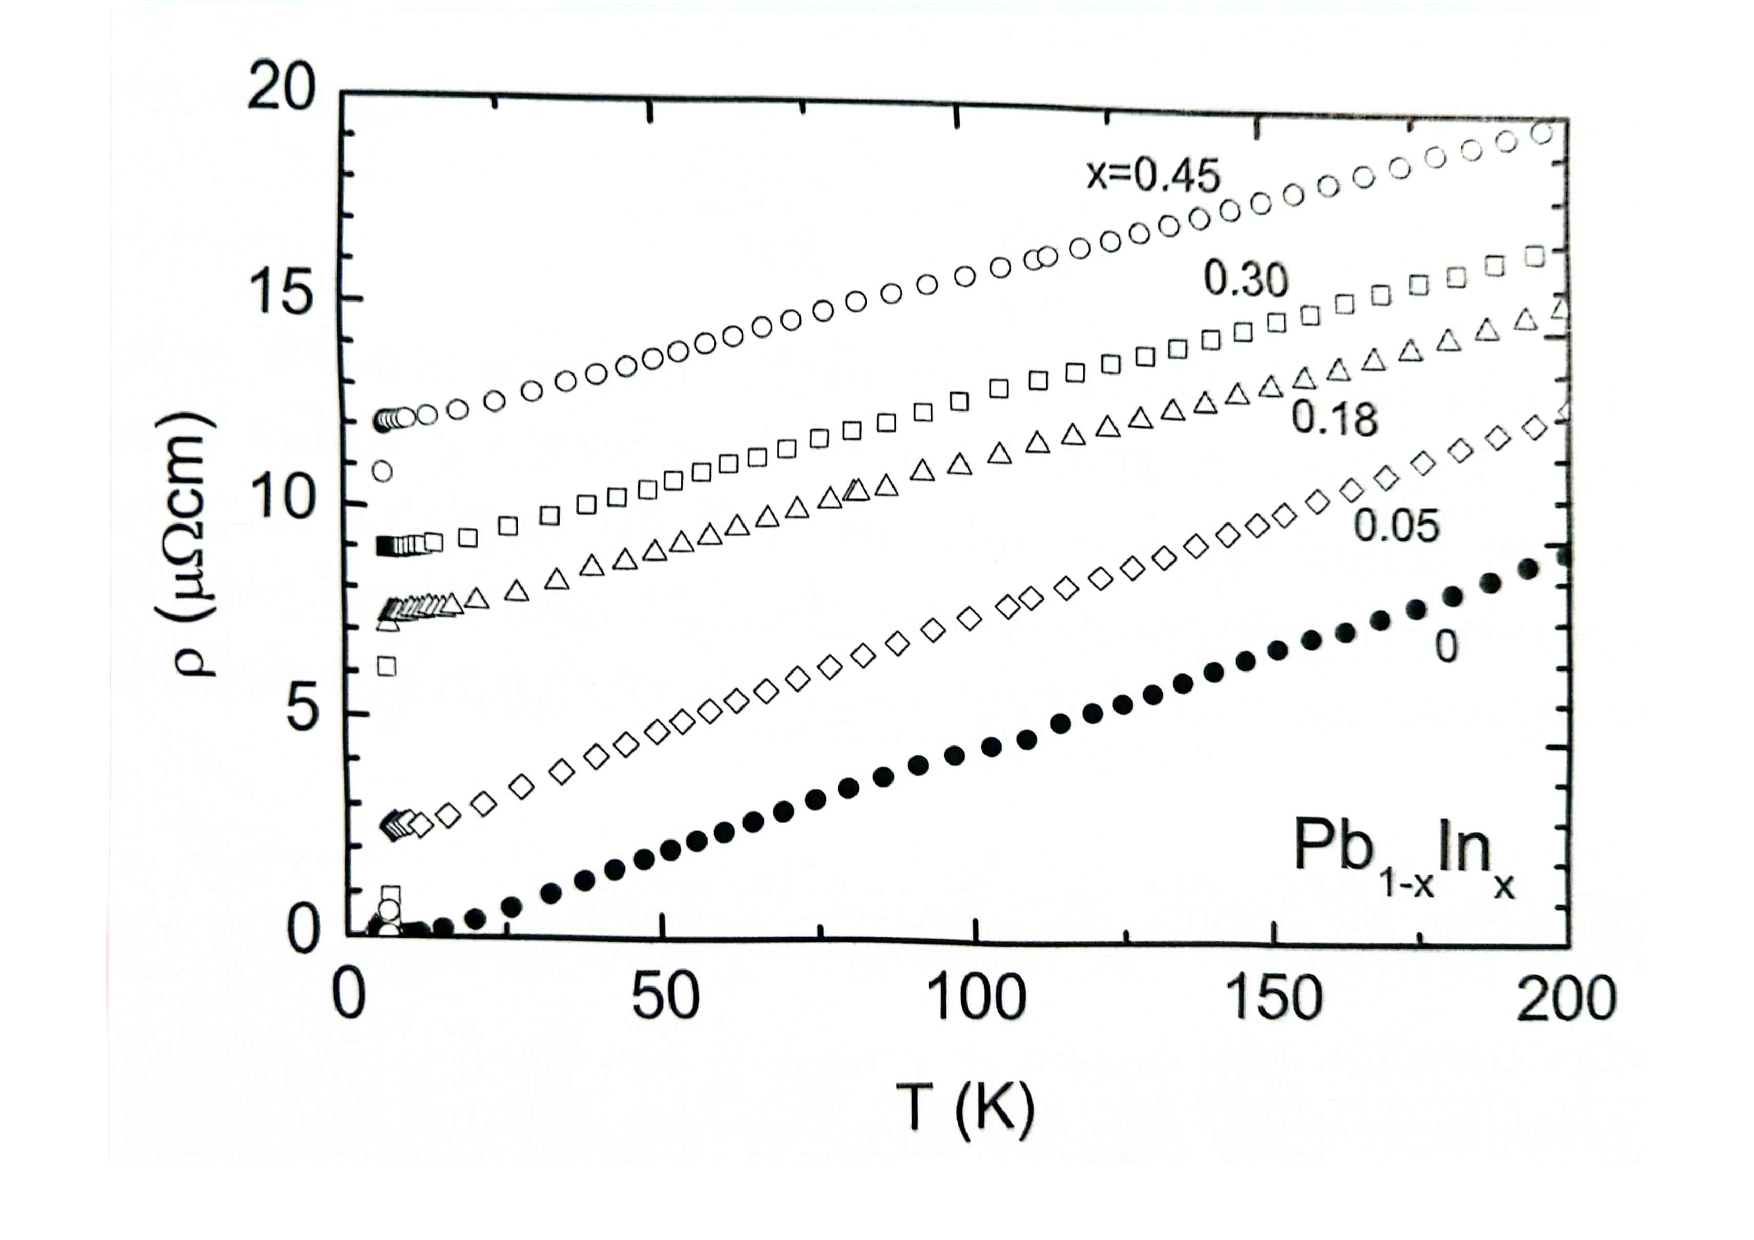
\includegraphics[scale=0.5]{Cuerpo/Ch_06/Fotos libro 6.pdf}
    \caption{Comprobación de la regla de Mathiessen con la resistividad de aleaciones de Pb-In. Al aumentar $x$ el desorden de la aleación y por tanto la contribución constante $\rho_{\text{def}}$ frente a $\rho_{\text{fon}} (T)$ que casi no cambia (nótese que la pendiente no varía). Es interesante que estas aleaciones son superconductores por debajo de $\sim 7$ K (veáse Capítulo \ref{Ch:11}).}
    \label{Fig:06-06}
\end{figure}  

\section{Conductivdad térmica electrónica}

\section{Ley de Wiedmann-Franz}

\section{Efecto Hall y magnetorresistividad}
\begin{figure}[h!] \centering
    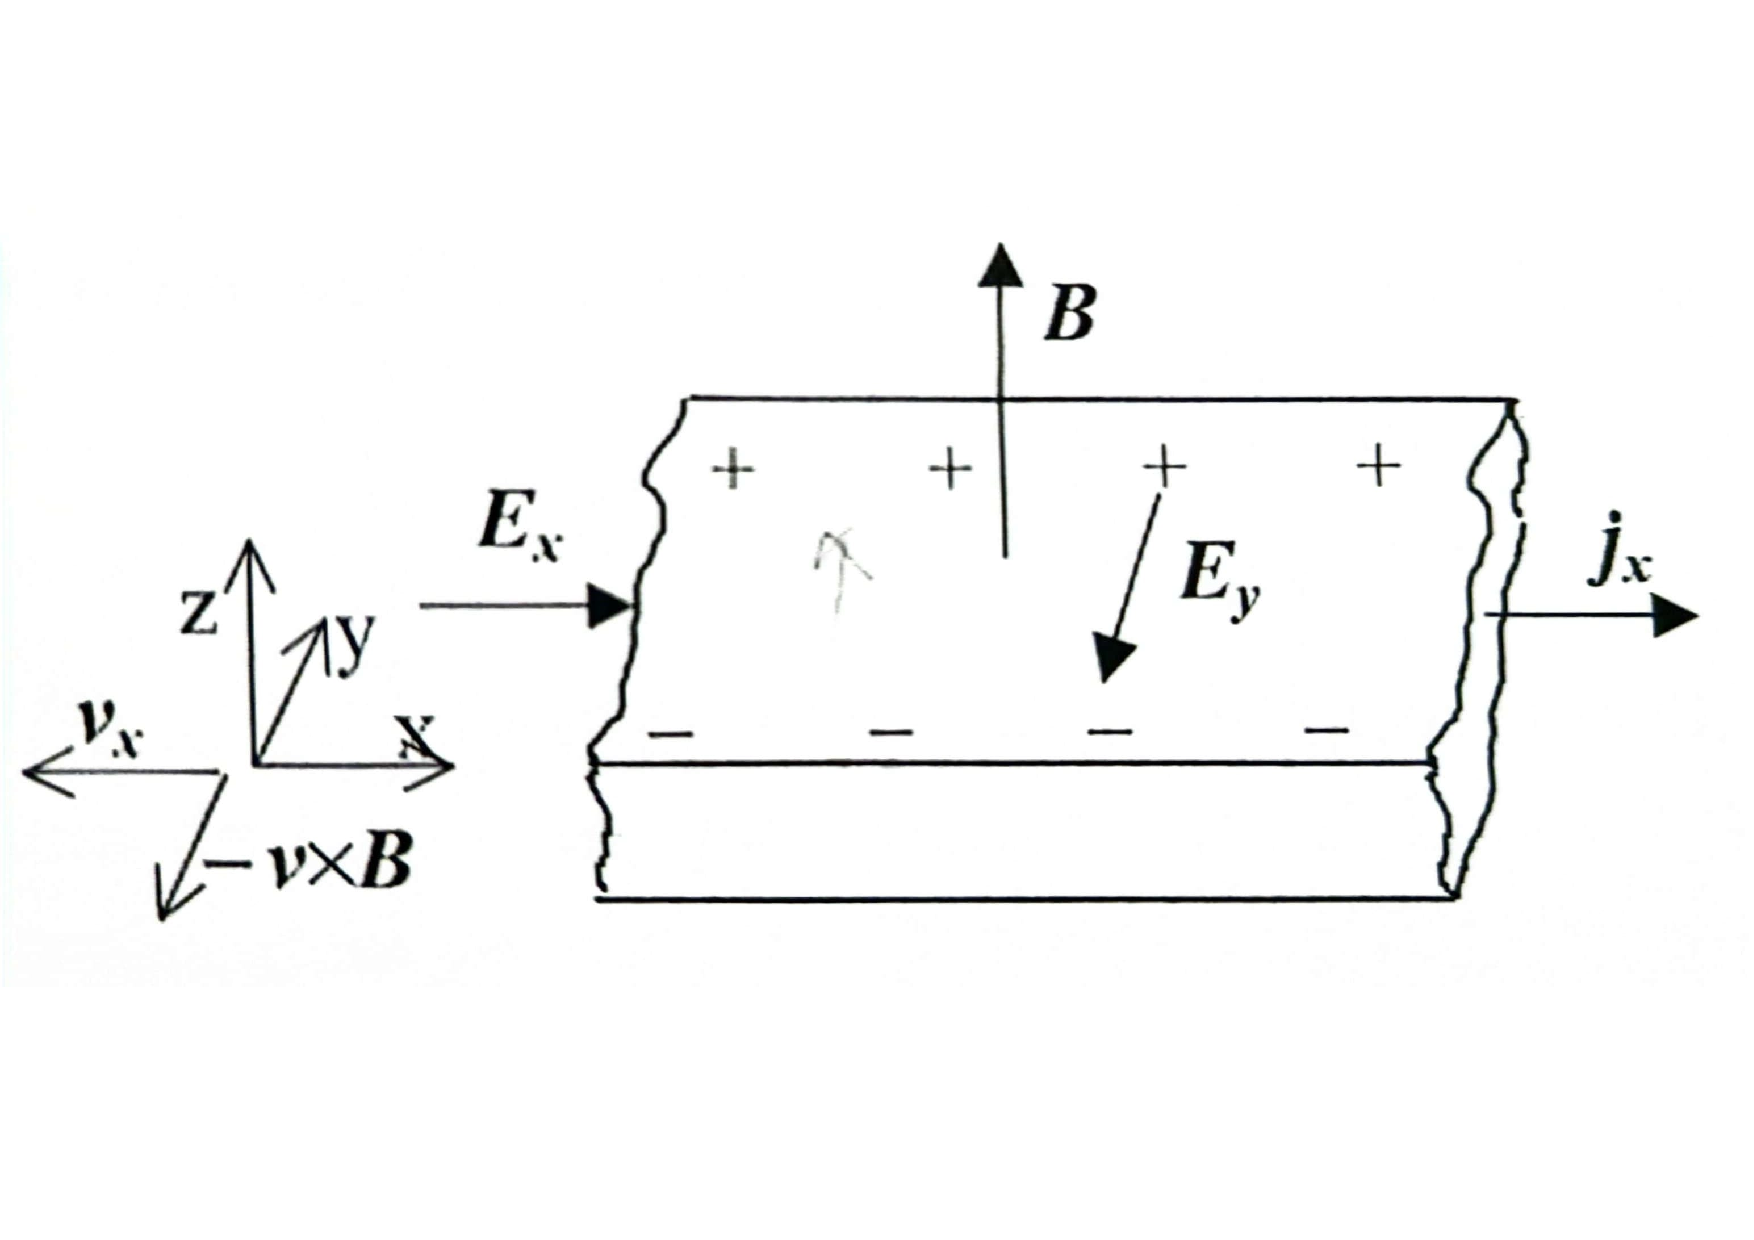
\includegraphics[scale=0.5]{Cuerpo/Ch_06/Fotos libro 7.pdf}
    \caption{Configuración experimental para comprobar el efecto Hall.}
    \label{Fig:06-07}
\end{figure}  


\section{Conductividad AC y propiedades ópticas}
